\chapter{Stellar Activity Modelling in Radial Velocity Time Series}
As discussed in Sect.~\ref{sect:activity}, there exists a multitude of physical
processes ongoing within the photospheres and chromospheres of active stars
which produce observable signatures with a variety of amplitudes and timescales
(see Table~\ref{table:activity}). The subsequent sections discuss a variety of
techniques which have been used to model and consequently mitigate the effects of
stellar activity in RV time series.

\section{An Overview of Techniques for Stellar Activity Mitigation}
\label{sect:methods}

\subsection{Stellar Activity as a Scalar Parameter}
Back in the day when the first giant exoplanets where being discovered with RVs,
typically treatment of stellar activity was implemented. The reason for this being
that the quality of the datasets at that time were insufficient to resolve the
temporal structure of RV activity for any but the most active stars. Many
observers however did report the root-mean-square (rms) of their RV residuals
following the removal of their best-fit planet model
\citep[e.g.][]{mayor95,butler96}. In
many cases, the residual rms was seen to exceed the characteristic RV measurement
uncertainty of the dataset and thus alluded to the presence of an additional
jitter signal which may or may not vary significantly with time. \\

In many of the following RV planet searches, the apparent jitter was
characterized by
an additive scalar $s$. The free parameter $s$ was used to characterize the level
of RV jitter as it was added in quadrature to the RV measurement uncertainties
when evaluating the objective function during any analysis equivalent or
analogous to a $\chi^2$-minimization routine. 


\subsection{Correlations with Activity Indicators}
Stellar RV observations are known to be affected by both planetary companions as
well as by stellar activity. Disentangling those signals in RV time series
therefore benefits significantly from ancillary time series which are sensitive
to stellar activity only \citep{boisse09}.
The classical implementation of de-correlation by
an activity indicator is to derive time series of one or many spectroscopic
activity indicators whose sampling is contemporaneous with the RVs and then
fitting an often linear relation between those datasets (Fig.~\ref{fig:corr}).
The relation, when fitted simultaneously with planetary solutions, allows the RVs
to be de-correlated jointly with the measurement of the planetary parameters.
This technique has been shown to be effective when the stellar rotation period
\prot{} is well constrained, the planetary orbital period is distinct from
\prot{,} the amplitude of the planetary signal exceeds that of the activity signal
by $\sim 30$\%, and the stellar rotation period is well sampled over multiple
cycles \citep{boisse11}. \\

\begin{figure}
  \centering
  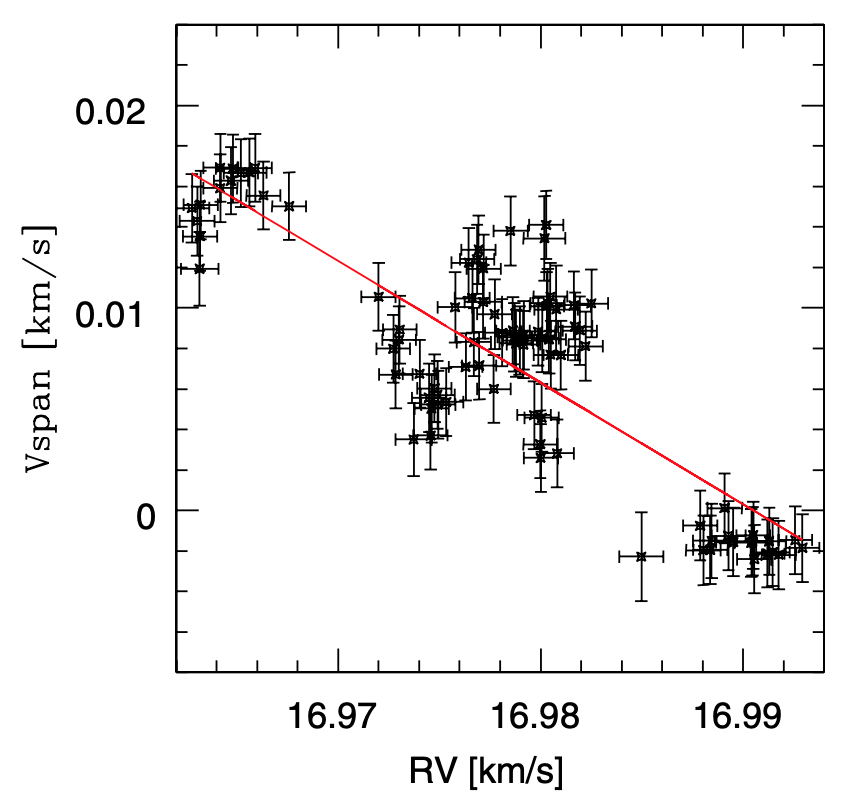
\includegraphics[width=.6\textwidth]{figures/vspan_rv.png}
  \caption{The correlation of the \vspan{} activity indicator with the RVs for the
    active Sun-like star HD 17051 from HARPS spectra. The solid line depicts the
    best-fit linear relation from least squares fitting. The fitted relation is
    used to de-correlate the RVs for the effects of stellar activity as probed by
    the \vspan{} time series. \citep[Image credit:][]{boisse11}.}
  \label{fig:corr}
\end{figure}

There exists a number of activity indicators which can be derived from the stellar
spectra. There definitions and physical motivations are summarized below.

\caii{} H\&K lines: 
For optical spectra with access to the \caii{} H and K lines
centered on 3968.47 \AA{} and 3933.66 \AA{,} the Mt. Wilson S-index is defined as

\begin{equation}
  \text{S-index} = \frac{\Psi_H + \Psi_K}{\Psi_B + \Psi_V}
\end{equation}

\noindent where $\Psi_H$ and $\Psi_K$ represent the narrowband
($\sim 1.1$ \AA{} wide) fluxes in the cores of the H and K lines of the \caii{}
doublet. The index is normalized by total flux in the $B$ and $V$ continuum bands
which are 20 \AA{} wide broad bands centered on 3900 and 4000 \AA{} respectively.

H$\alpha$: ...
Similar emission line features may also be used as activity indicators depending
on the accessible wavelengths of the spectrograph (e.g. \hei{,} \nai{,} etc).

Vspan:
\citep{queloz01}

FWHM:

BIS:


\citep{boisse09,boisse11}

\subsection{Photometric Modelling: the FF' Method }
\citep{aigrain12}

\subsection{Pre-whitening}
\citep{queloz09}

\subsection{Physical Models of Active Regions}
\citep{dumusque14}

\subsection{Deterministic Model Fitting}
\citep{sarkis18}


\section{Point-form Thesis: Stellar Activity Modelling in Radial Velocity
  Time Series}
\begin{itemize}
\renewcommand\labelitemi{--}
\item~\ref{sect:methods} \textbf{An Overview of Techniques for Stellar Activity
Mitigation}:
\end{itemize}
